\documentclass[twoside]{article}

% Packages required by doxygen
\usepackage{calc}
\usepackage{doxygen}
\usepackage{graphicx}
\usepackage[utf8]{inputenc}
\usepackage{makeidx}
\usepackage{multicol}
\usepackage{multirow}
\usepackage{textcomp}
\usepackage[table]{xcolor}

% Font selection
\usepackage[T1]{fontenc}
\usepackage{mathptmx}
\usepackage[scaled=.90]{helvet}
\usepackage{courier}
\usepackage{amssymb}
\usepackage{sectsty}
\renewcommand{\familydefault}{\sfdefault}
\allsectionsfont{%
  \fontseries{bc}\selectfont%
  \color{darkgray}%
}
\renewcommand{\DoxyLabelFont}{%
  \fontseries{bc}\selectfont%
  \color{darkgray}%
}

% Page & text layout
\usepackage{geometry}
\geometry{%
  a4paper,%
  top=2.5cm,%
  bottom=2.5cm,%
  left=2.5cm,%
  right=2.5cm%
}
\tolerance=750
\hfuzz=15pt
\hbadness=750
\setlength{\emergencystretch}{15pt}
\setlength{\parindent}{0cm}
\setlength{\parskip}{0.2cm}
\makeatletter
\renewcommand{\paragraph}{%
  \@startsection{paragraph}{4}{0ex}{-1.0ex}{1.0ex}{%
    \normalfont\normalsize\bfseries\SS@parafont%
  }%
}
\renewcommand{\subparagraph}{%
  \@startsection{subparagraph}{5}{0ex}{-1.0ex}{1.0ex}{%
    \normalfont\normalsize\bfseries\SS@subparafont%
  }%
}
\makeatother

% Headers & footers
\usepackage{fancyhdr}
\pagestyle{fancyplain}
\fancyhead[LE]{\fancyplain{}{\bfseries\thepage}}
\fancyhead[CE]{\fancyplain{}{}}
\fancyhead[RE]{\fancyplain{}{\bfseries\leftmark}}
\fancyhead[LO]{\fancyplain{}{\bfseries\rightmark}}
\fancyhead[CO]{\fancyplain{}{}}
\fancyhead[RO]{\fancyplain{}{\bfseries\thepage}}
\fancyfoot[LE]{\fancyplain{}{}}
\fancyfoot[CE]{\fancyplain{}{}}
\fancyfoot[RE]{\fancyplain{}{\bfseries\scriptsize Generated on Sun Mar 15 2015 18\-:40\-:51 for Zadanie 2 by Doxygen }}
\fancyfoot[LO]{\fancyplain{}{\bfseries\scriptsize Generated on Sun Mar 15 2015 18\-:40\-:51 for Zadanie 2 by Doxygen }}
\fancyfoot[CO]{\fancyplain{}{}}
\fancyfoot[RO]{\fancyplain{}{}}
\renewcommand{\footrulewidth}{0.4pt}
\renewcommand{\sectionmark}[1]{%
  \markright{\thesection\ #1}%
}

% Indices & bibliography
\usepackage{natbib}
\usepackage[titles]{tocloft}
\setcounter{tocdepth}{3}
\setcounter{secnumdepth}{5}
\makeindex

% Hyperlinks (required, but should be loaded last)
\usepackage{ifpdf}
\ifpdf
  \usepackage[pdftex,pagebackref=true]{hyperref}
\else
  \usepackage[ps2pdf,pagebackref=true]{hyperref}
\fi
\hypersetup{%
  colorlinks=true,%
  linkcolor=blue,%
  citecolor=blue,%
  unicode%
}

% Custom commands
\newcommand{\clearemptydoublepage}{%
  \newpage{\pagestyle{empty}\cleardoublepage}%
}


%===== C O N T E N T S =====

\begin{document}

% Titlepage & ToC
\hypersetup{pageanchor=false}
\pagenumbering{roman}
\begin{titlepage}
\vspace*{7cm}
\begin{center}%
{\Large Zadanie 2 }\\
\vspace*{1cm}
{\large Generated by Doxygen 1.8.6}\\
\vspace*{0.5cm}
{\small Sun Mar 15 2015 18:40:51}\\
\end{center}
\end{titlepage}
\tableofcontents
\pagenumbering{arabic}
\hypersetup{pageanchor=true}

%--- Begin generated contents ---
\section{Class Index}
\section{Class List}
Here are the classes, structs, unions and interfaces with brief descriptions\+:\begin{DoxyCompactList}
\item\contentsline{section}{\hyperlink{a00001}{Array\+Lista} \\*Klasa \hyperlink{a00001}{Array\+Lista} }{\pageref{a00001}}{}
\item\contentsline{section}{\hyperlink{a00002}{Benchmarker} \\*Klasa \hyperlink{a00002}{Benchmarker} }{\pageref{a00002}}{}
\item\contentsline{section}{\hyperlink{a00003}{Hasz\+Tab} \\*Klasa \hyperlink{a00003}{Hasz\+Tab} }{\pageref{a00003}}{}
\item\contentsline{section}{\hyperlink{a00004}{Kolejka} \\*Klasa \hyperlink{a00004}{Kolejka} }{\pageref{a00004}}{}
\item\contentsline{section}{\hyperlink{a00005}{Lista} \\*Klasa \hyperlink{a00005}{Lista} }{\pageref{a00005}}{}
\item\contentsline{section}{\hyperlink{a00006}{Stos} \\*Klasa \hyperlink{a00006}{Stos} }{\pageref{a00006}}{}
\end{DoxyCompactList}

\section{File Index}
\subsection{File List}
Here is a list of all files with brief descriptions\-:\begin{DoxyCompactList}
\item\contentsline{section}{\hyperlink{a00002}{Benchmark.\-cpp} \\*Metody klasy \hyperlink{a00001}{Benchmarker} }{\pageref{a00002}}{}
\item\contentsline{section}{\hyperlink{a00003}{Benchmark.\-hh} \\*Definicja klasy Benchmark }{\pageref{a00003}}{}
\item\contentsline{section}{\hyperlink{a00004}{main.\-cpp} \\*Modul glowny }{\pageref{a00004}}{}
\end{DoxyCompactList}

\section{Class Documentation}
\hypertarget{a00001}{\subsection{Benchmarker Class Reference}
\label{a00001}\index{Benchmarker@{Benchmarker}}
}


Klasa benchmarku.  




{\ttfamily \#include $<$Benchmark.\-hh$>$}

\subsubsection*{Public Member Functions}
\begin{DoxyCompactItemize}
\item 
\hyperlink{a00001_aab7e84d7ce96b1a26eee22f9fc11a55a}{Benchmarker} ()
\begin{DoxyCompactList}\small\item\em Konstruktor bezparametryczny . \end{DoxyCompactList}\item 
\hyperlink{a00001_a2ef2105cab075e03500d057780c7694e}{$\sim$\-Benchmarker} ()
\begin{DoxyCompactList}\small\item\em Destruktor bezparametryczny. \end{DoxyCompactList}\item 
long long int \hyperlink{a00001_af0281a2fc6e1cb2e0041d548f6163fee}{testuj} (int $\ast$, int $\ast$, int, int)
\begin{DoxyCompactList}\small\item\em Metoda przeprowadzajaca sprawdzenie czasy dzialania funkcji. sprawdzienie czasu dzialania mnozenia kazdego elementu tablicy razy 2. \end{DoxyCompactList}\item 
int $\ast$ \hyperlink{a00001_a917b8efeea3b8a82882be68e490548e8}{generuj\-\_\-dane} (int)
\end{DoxyCompactItemize}


\subsubsection{Detailed Description}
Klasa benchmarku. 

\subsubsection{Constructor \& Destructor Documentation}
\hypertarget{a00001_aab7e84d7ce96b1a26eee22f9fc11a55a}{\index{Benchmarker@{Benchmarker}!Benchmarker@{Benchmarker}}
\index{Benchmarker@{Benchmarker}!Benchmarker@{Benchmarker}}
\paragraph[{Benchmarker}]{\setlength{\rightskip}{0pt plus 5cm}Benchmarker\-::\-Benchmarker (
\begin{DoxyParamCaption}
{}
\end{DoxyParamCaption}
)}}\label{a00001_aab7e84d7ce96b1a26eee22f9fc11a55a}


Konstruktor bezparametryczny . 

\hypertarget{a00001_a2ef2105cab075e03500d057780c7694e}{\index{Benchmarker@{Benchmarker}!$\sim$\-Benchmarker@{$\sim$\-Benchmarker}}
\index{$\sim$\-Benchmarker@{$\sim$\-Benchmarker}!Benchmarker@{Benchmarker}}
\paragraph[{$\sim$\-Benchmarker}]{\setlength{\rightskip}{0pt plus 5cm}Benchmarker\-::$\sim$\-Benchmarker (
\begin{DoxyParamCaption}
{}
\end{DoxyParamCaption}
)}}\label{a00001_a2ef2105cab075e03500d057780c7694e}


Destruktor bezparametryczny. 



\subsubsection{Member Function Documentation}
\hypertarget{a00001_a917b8efeea3b8a82882be68e490548e8}{\index{Benchmarker@{Benchmarker}!generuj\-\_\-dane@{generuj\-\_\-dane}}
\index{generuj\-\_\-dane@{generuj\-\_\-dane}!Benchmarker@{Benchmarker}}
\paragraph[{generuj\-\_\-dane}]{\setlength{\rightskip}{0pt plus 5cm}int$\ast$ Benchmarker\-::generuj\-\_\-dane (
\begin{DoxyParamCaption}
\item[{int}]{}
\end{DoxyParamCaption}
)}}\label{a00001_a917b8efeea3b8a82882be68e490548e8}
\hypertarget{a00001_af0281a2fc6e1cb2e0041d548f6163fee}{\index{Benchmarker@{Benchmarker}!testuj@{testuj}}
\index{testuj@{testuj}!Benchmarker@{Benchmarker}}
\paragraph[{testuj}]{\setlength{\rightskip}{0pt plus 5cm}long long int Benchmarker\-::testuj (
\begin{DoxyParamCaption}
\item[{int $\ast$}]{tab, }
\item[{int $\ast$}]{dane, }
\item[{int}]{liczba\-\_\-przejsc, }
\item[{int}]{liczba\-\_\-danych}
\end{DoxyParamCaption}
)}}\label{a00001_af0281a2fc6e1cb2e0041d548f6163fee}


Metoda przeprowadzajaca sprawdzenie czasy dzialania funkcji. sprawdzienie czasu dzialania mnozenia kazdego elementu tablicy razy 2. 


\begin{DoxyParams}{Parameters}
{\em tab} & -\/ typu int$\ast$, wskaznik na tablice z wartosciami. \\
\hline
{\em dane} & -\/ typu int$\ast$, wskaznik na tablice z danymi generowanymi. \\
\hline
{\em liczba\-\_\-przejsc} & -\/ typu int, liczba przejsc przez dane. \\
\hline
{\em liczba\-\_\-danych} & -\/ typu int, liczba danych w tablicy. \\
\hline
\end{DoxyParams}
\begin{DoxyReturn}{Returns}
czas\-\_\-calkowity\-\_\-usredniony -\/ typu int, czas sredni dzialania funkcji. 
\end{DoxyReturn}


The documentation for this class was generated from the following files\-:\begin{DoxyCompactItemize}
\item 
\hyperlink{a00003}{Benchmark.\-hh}\item 
\hyperlink{a00002}{Benchmark.\-cpp}\end{DoxyCompactItemize}

\hypertarget{a00002}{}\section{Algorytm1 Class Reference}
\label{a00002}\index{Algorytm1@{Algorytm1}}


Klasa \hyperlink{a00002}{Algorytm1}.  




{\ttfamily \#include $<$Algorytm1.\+hh$>$}



Inheritance diagram for Algorytm1\+:
\nopagebreak
\begin{figure}[H]
\begin{center}
\leavevmode
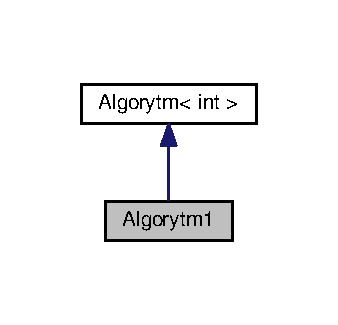
\includegraphics[width=162pt]{a00118}
\end{center}
\end{figure}


Collaboration diagram for Algorytm1\+:
\nopagebreak
\begin{figure}[H]
\begin{center}
\leavevmode
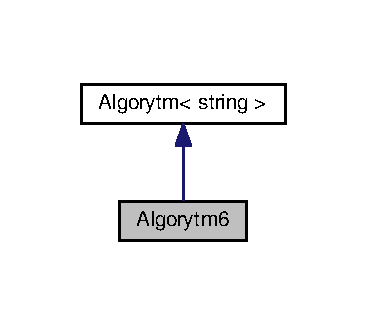
\includegraphics[width=162pt]{a00119}
\end{center}
\end{figure}
\subsection*{Public Member Functions}
\begin{DoxyCompactItemize}
\item 
\hyperlink{a00002_abb461ae4b741a82619039d789e0d2b0e}{$\sim$\+Algorytm1} ()
\item 
void \hyperlink{a00002_a0a9f86a1cf3b22e273042010d3a7d00f}{alokujdane} (\hyperlink{a00019}{Zasobnik}$<$ int $>$ $\ast$, int $\ast$, int)
\begin{DoxyCompactList}\small\item\em Metoda alokujaca na zasobniku dane. \end{DoxyCompactList}\item 
void \hyperlink{a00002_aca10f2c6923337e0ab928338e8989417}{wykonajalgorytm} (\hyperlink{a00019}{Zasobnik}$<$ int $>$ $\ast$, int $\ast$, int)
\begin{DoxyCompactList}\small\item\em Metoda wykonujaca konkretny algorytm. \end{DoxyCompactList}\end{DoxyCompactItemize}


\subsection{Detailed Description}
Klasa \hyperlink{a00002}{Algorytm1}. 

\subsection{Constructor \& Destructor Documentation}
\hypertarget{a00002_abb461ae4b741a82619039d789e0d2b0e}{}\index{Algorytm1@{Algorytm1}!````~Algorytm1@{$\sim$\+Algorytm1}}
\index{````~Algorytm1@{$\sim$\+Algorytm1}!Algorytm1@{Algorytm1}}
\subsubsection[{$\sim$\+Algorytm1}]{\setlength{\rightskip}{0pt plus 5cm}Algorytm1\+::$\sim$\+Algorytm1 (
\begin{DoxyParamCaption}
{}
\end{DoxyParamCaption}
)\hspace{0.3cm}{\ttfamily [inline]}}\label{a00002_abb461ae4b741a82619039d789e0d2b0e}


\subsection{Member Function Documentation}
\hypertarget{a00002_a0a9f86a1cf3b22e273042010d3a7d00f}{}\index{Algorytm1@{Algorytm1}!alokujdane@{alokujdane}}
\index{alokujdane@{alokujdane}!Algorytm1@{Algorytm1}}
\subsubsection[{alokujdane}]{\setlength{\rightskip}{0pt plus 5cm}void Algorytm1\+::alokujdane (
\begin{DoxyParamCaption}
\item[{{\bf Zasobnik}$<$ int $>$ $\ast$}]{Tab, }
\item[{int $\ast$}]{dane, }
\item[{int}]{liczba\+\_\+danych}
\end{DoxyParamCaption}
)\hspace{0.3cm}{\ttfamily [virtual]}}\label{a00002_a0a9f86a1cf3b22e273042010d3a7d00f}


Metoda alokujaca na zasobniku dane. 


\begin{DoxyParams}{Parameters}
{\em Tab} & -\/ typu Zasobnik$<$\+T$>$$\ast$, implementacja zasobnika \\
\hline
{\em dane} & -\/ typu T$\ast$, dane wygenerowane dla implementacji \\
\hline
{\em liczba\+\_\+danych} & -\/ typu int, liczba danych dla zasobnika \\
\hline
\end{DoxyParams}


Implements \hyperlink{a00001_a1e83fd87a20fd0a13ebbf1c81e457b61}{Algorytm$<$ int $>$}.

\hypertarget{a00002_aca10f2c6923337e0ab928338e8989417}{}\index{Algorytm1@{Algorytm1}!wykonajalgorytm@{wykonajalgorytm}}
\index{wykonajalgorytm@{wykonajalgorytm}!Algorytm1@{Algorytm1}}
\subsubsection[{wykonajalgorytm}]{\setlength{\rightskip}{0pt plus 5cm}void Algorytm1\+::wykonajalgorytm (
\begin{DoxyParamCaption}
\item[{{\bf Zasobnik}$<$ int $>$ $\ast$}]{Tab, }
\item[{int $\ast$}]{dane, }
\item[{int}]{liczba\+\_\+danych}
\end{DoxyParamCaption}
)\hspace{0.3cm}{\ttfamily [virtual]}}\label{a00002_aca10f2c6923337e0ab928338e8989417}


Metoda wykonujaca konkretny algorytm. 


\begin{DoxyParams}{Parameters}
{\em Tab} & -\/ typu Zasobnik$<$\+T$>$$\ast$, implementacja zasobnika \\
\hline
{\em dane} & -\/ typu T$\ast$, dane wygenerowane dla implementacji \\
\hline
{\em liczba\+\_\+danych} & -\/ typu int, liczba danych dla zasobnika \\
\hline
\end{DoxyParams}


Implements \hyperlink{a00001_ae97a52b1a728be1a819c9e9815f424e7}{Algorytm$<$ int $>$}.



The documentation for this class was generated from the following files\+:\begin{DoxyCompactItemize}
\item 
\hyperlink{a00021}{Algorytm1.\+hh}\item 
\hyperlink{a00020}{Algorytm1.\+cpp}\end{DoxyCompactItemize}

\hypertarget{a00003}{}\section{Kolejka Class Reference}
\label{a00003}\index{Kolejka@{Kolejka}}


Klasa \hyperlink{a00003}{Kolejka}.  




{\ttfamily \#include $<$Kolejka.\+hh$>$}

\subsection*{Public Member Functions}
\begin{DoxyCompactItemize}
\item 
\hyperlink{a00003_a37c886fdc73dce62b04da0381dec5484}{Kolejka} ()
\begin{DoxyCompactList}\small\item\em Konstruktor bezparametryczny. Konstruktor inicjalizujacy straznika\+\_\+poczatek i straznika\+\_\+koniec kolejki wartosciami N\+U\+L\+L , oraz rozmiar kolejki wartoscia 0. \end{DoxyCompactList}\item 
\hyperlink{a00003_a352f86ff08cd47be6c35c60bb0f873a6}{$\sim$\+Kolejka} ()
\begin{DoxyCompactList}\small\item\em Destruktor bezparametryczny kolejki. \end{DoxyCompactList}\item 
void \hyperlink{a00003_abdd1c95eb88905167ec26658b6b76611}{push} (int)
\begin{DoxyCompactList}\small\item\em Metoda umieszczajaca element na koncu kolejki. Metoda inkrementuje rozmiar podczas umieszczania elementu w kolejce. \end{DoxyCompactList}\item 
int \hyperlink{a00003_aa99d7c7459116c2331b301637b45b666}{pop} ()
\begin{DoxyCompactList}\small\item\em Metoda zdejmujaca element z poczatku kolejki. Metoda dekrementuje rozmiar przy zdejmowaniu elementu. \end{DoxyCompactList}\item 
int \hyperlink{a00003_a82920d7b90e967a4d5e175a20fe6de68}{size} ()
\begin{DoxyCompactList}\small\item\em Metoda zwracajaca wielkosc kolejki. \end{DoxyCompactList}\end{DoxyCompactItemize}


\subsection{Detailed Description}
Klasa \hyperlink{a00003}{Kolejka}. 

\subsection{Constructor \& Destructor Documentation}
\hypertarget{a00003_a37c886fdc73dce62b04da0381dec5484}{}\index{Kolejka@{Kolejka}!Kolejka@{Kolejka}}
\index{Kolejka@{Kolejka}!Kolejka@{Kolejka}}
\subsubsection[{Kolejka}]{\setlength{\rightskip}{0pt plus 5cm}Kolejka\+::\+Kolejka (
\begin{DoxyParamCaption}
{}
\end{DoxyParamCaption}
)}\label{a00003_a37c886fdc73dce62b04da0381dec5484}


Konstruktor bezparametryczny. Konstruktor inicjalizujacy straznika\+\_\+poczatek i straznika\+\_\+koniec kolejki wartosciami N\+U\+L\+L , oraz rozmiar kolejki wartoscia 0. 

\hypertarget{a00003_a352f86ff08cd47be6c35c60bb0f873a6}{}\index{Kolejka@{Kolejka}!````~Kolejka@{$\sim$\+Kolejka}}
\index{````~Kolejka@{$\sim$\+Kolejka}!Kolejka@{Kolejka}}
\subsubsection[{$\sim$\+Kolejka}]{\setlength{\rightskip}{0pt plus 5cm}Kolejka\+::$\sim$\+Kolejka (
\begin{DoxyParamCaption}
{}
\end{DoxyParamCaption}
)}\label{a00003_a352f86ff08cd47be6c35c60bb0f873a6}


Destruktor bezparametryczny kolejki. 



\subsection{Member Function Documentation}
\hypertarget{a00003_aa99d7c7459116c2331b301637b45b666}{}\index{Kolejka@{Kolejka}!pop@{pop}}
\index{pop@{pop}!Kolejka@{Kolejka}}
\subsubsection[{pop}]{\setlength{\rightskip}{0pt plus 5cm}int Kolejka\+::pop (
\begin{DoxyParamCaption}
{}
\end{DoxyParamCaption}
)}\label{a00003_aa99d7c7459116c2331b301637b45b666}


Metoda zdejmujaca element z poczatku kolejki. Metoda dekrementuje rozmiar przy zdejmowaniu elementu. 

\begin{DoxyReturn}{Returns}
wartosc -\/ typu int, wartosc zdejmowana z kolejki. 
\end{DoxyReturn}
\hypertarget{a00003_abdd1c95eb88905167ec26658b6b76611}{}\index{Kolejka@{Kolejka}!push@{push}}
\index{push@{push}!Kolejka@{Kolejka}}
\subsubsection[{push}]{\setlength{\rightskip}{0pt plus 5cm}void Kolejka\+::push (
\begin{DoxyParamCaption}
\item[{int}]{wartosc}
\end{DoxyParamCaption}
)}\label{a00003_abdd1c95eb88905167ec26658b6b76611}


Metoda umieszczajaca element na koncu kolejki. Metoda inkrementuje rozmiar podczas umieszczania elementu w kolejce. 


\begin{DoxyParams}{Parameters}
{\em wartosc} & -\/ typu int, wartosc umieszczana na koncu kolejki. \\
\hline
\end{DoxyParams}
\hypertarget{a00003_a82920d7b90e967a4d5e175a20fe6de68}{}\index{Kolejka@{Kolejka}!size@{size}}
\index{size@{size}!Kolejka@{Kolejka}}
\subsubsection[{size}]{\setlength{\rightskip}{0pt plus 5cm}int Kolejka\+::size (
\begin{DoxyParamCaption}
{}
\end{DoxyParamCaption}
)}\label{a00003_a82920d7b90e967a4d5e175a20fe6de68}


Metoda zwracajaca wielkosc kolejki. 

\begin{DoxyReturn}{Returns}
rozmiar -\/ typu int,rozmiar kolejki. 
\end{DoxyReturn}


The documentation for this class was generated from the following files\+:\begin{DoxyCompactItemize}
\item 
\hyperlink{a00011}{Kolejka.\+hh}\item 
\hyperlink{a00010}{Kolejka.\+cpp}\end{DoxyCompactItemize}

\hypertarget{a00004}{\subsection{main.\-cpp File Reference}
\label{a00004}\index{main.\-cpp@{main.\-cpp}}
}


Modul glowny.  


{\ttfamily \#include $<$cstdlib$>$}\\*
{\ttfamily \#include $<$iostream$>$}\\*
{\ttfamily \#include $<$fstream$>$}\\*
{\ttfamily \#include \char`\"{}Benchmark.\-hh\char`\"{}}\\*
Include dependency graph for main.\-cpp\-:
\nopagebreak
\begin{figure}[H]
\begin{center}
\leavevmode
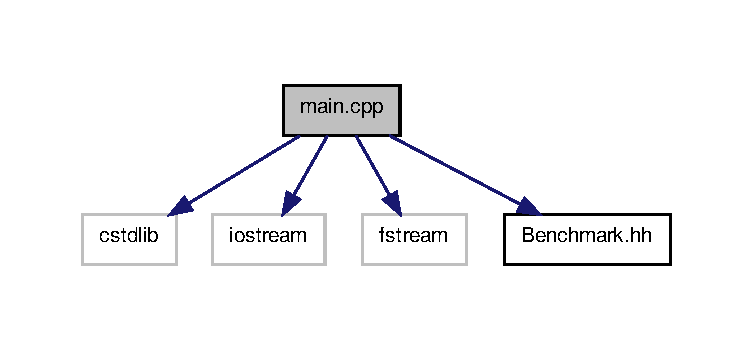
\includegraphics[width=350pt]{a00009}
\end{center}
\end{figure}
\subsubsection*{Functions}
\begin{DoxyCompactItemize}
\item 
int \hyperlink{a00004_ae66f6b31b5ad750f1fe042a706a4e3d4}{main} ()
\begin{DoxyCompactList}\small\item\em Funkcja glowna programu. \end{DoxyCompactList}\end{DoxyCompactItemize}


\subsubsection{Detailed Description}
Modul glowny. Plik zawiera funkcje main. 

\subsubsection{Function Documentation}
\hypertarget{a00004_ae66f6b31b5ad750f1fe042a706a4e3d4}{\index{main.\-cpp@{main.\-cpp}!main@{main}}
\index{main@{main}!main.cpp@{main.\-cpp}}
\paragraph[{main}]{\setlength{\rightskip}{0pt plus 5cm}int main (
\begin{DoxyParamCaption}
{}
\end{DoxyParamCaption}
)}}\label{a00004_ae66f6b31b5ad750f1fe042a706a4e3d4}


Funkcja glowna programu. 



Here is the call graph for this function\-:
\nopagebreak
\begin{figure}[H]
\begin{center}
\leavevmode
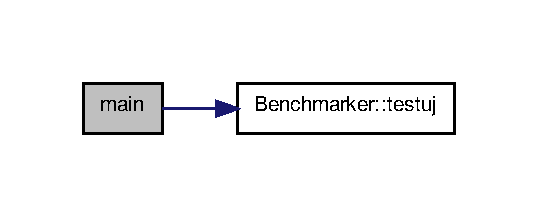
\includegraphics[width=258pt]{a00004_ae66f6b31b5ad750f1fe042a706a4e3d4_cgraph}
\end{center}
\end{figure}



\section{File Documentation}
\hypertarget{a00005}{\section{Stos Class Reference}
\label{a00005}\index{Stos@{Stos}}
}


Klasa \hyperlink{a00005}{Stos}.  




{\ttfamily \#include $<$Stos.\-hh$>$}

\subsection*{Public Member Functions}
\begin{DoxyCompactItemize}
\item 
\hyperlink{a00005_a1de3b50386d5dfb56ddece17d0ea2389}{Stos} ()
\begin{DoxyCompactList}\small\item\em Konstruktor bezparametryczny. Konstruktor inicjalizujacy straznika stosu wartoscia N\-U\-L\-L ,oraz rozmiar wartoscia 0. \end{DoxyCompactList}\item 
\hyperlink{a00005_af9a198e2540e18adcc0b5259105fd78e}{$\sim$\-Stos} ()
\begin{DoxyCompactList}\small\item\em Destruktor bezparametryczny stosu. \end{DoxyCompactList}\item 
void \hyperlink{a00005_afe381df2afa35f3d122ca180300005dd}{push} (int)
\begin{DoxyCompactList}\small\item\em Metoda umieszczajaca element na stosie Metoda inkrementuje rozmiar podczas umieszczania elementu na stosie. \end{DoxyCompactList}\item 
int \hyperlink{a00005_aabb14b8a389c55da6e2b50fbb179ed56}{pop} ()
\begin{DoxyCompactList}\small\item\em Metoda zdejmujaca element ze stosu. Metoda dekrementuje rozmiar przy zdejmowaniu ze stosu. \end{DoxyCompactList}\item 
int \hyperlink{a00005_a696195d5125d9bbe6b491bc5985f9461}{size} ()
\begin{DoxyCompactList}\small\item\em Metoda zwracajaca wielkosc stosu. \end{DoxyCompactList}\end{DoxyCompactItemize}


\subsection{Detailed Description}
Klasa \hyperlink{a00005}{Stos}. 

\subsection{Constructor \& Destructor Documentation}
\hypertarget{a00005_a1de3b50386d5dfb56ddece17d0ea2389}{\index{Stos@{Stos}!Stos@{Stos}}
\index{Stos@{Stos}!Stos@{Stos}}
\subsubsection[{Stos}]{\setlength{\rightskip}{0pt plus 5cm}Stos\-::\-Stos (
\begin{DoxyParamCaption}
{}
\end{DoxyParamCaption}
)}}\label{a00005_a1de3b50386d5dfb56ddece17d0ea2389}


Konstruktor bezparametryczny. Konstruktor inicjalizujacy straznika stosu wartoscia N\-U\-L\-L ,oraz rozmiar wartoscia 0. 

\hypertarget{a00005_af9a198e2540e18adcc0b5259105fd78e}{\index{Stos@{Stos}!$\sim$\-Stos@{$\sim$\-Stos}}
\index{$\sim$\-Stos@{$\sim$\-Stos}!Stos@{Stos}}
\subsubsection[{$\sim$\-Stos}]{\setlength{\rightskip}{0pt plus 5cm}Stos\-::$\sim$\-Stos (
\begin{DoxyParamCaption}
{}
\end{DoxyParamCaption}
)}}\label{a00005_af9a198e2540e18adcc0b5259105fd78e}


Destruktor bezparametryczny stosu. 



\subsection{Member Function Documentation}
\hypertarget{a00005_aabb14b8a389c55da6e2b50fbb179ed56}{\index{Stos@{Stos}!pop@{pop}}
\index{pop@{pop}!Stos@{Stos}}
\subsubsection[{pop}]{\setlength{\rightskip}{0pt plus 5cm}int Stos\-::pop (
\begin{DoxyParamCaption}
{}
\end{DoxyParamCaption}
)}}\label{a00005_aabb14b8a389c55da6e2b50fbb179ed56}


Metoda zdejmujaca element ze stosu. Metoda dekrementuje rozmiar przy zdejmowaniu ze stosu. 

\begin{DoxyReturn}{Returns}
wartosc -\/ typu int, wartosc zdejmowana ze stosu. 
\end{DoxyReturn}
\hypertarget{a00005_afe381df2afa35f3d122ca180300005dd}{\index{Stos@{Stos}!push@{push}}
\index{push@{push}!Stos@{Stos}}
\subsubsection[{push}]{\setlength{\rightskip}{0pt plus 5cm}void Stos\-::push (
\begin{DoxyParamCaption}
\item[{int}]{wartosc}
\end{DoxyParamCaption}
)}}\label{a00005_afe381df2afa35f3d122ca180300005dd}


Metoda umieszczajaca element na stosie Metoda inkrementuje rozmiar podczas umieszczania elementu na stosie. 


\begin{DoxyParams}{Parameters}
{\em wartosc} & -\/ typu int, wartosc umieszczana na stosie. \\
\hline
\end{DoxyParams}
\hypertarget{a00005_a696195d5125d9bbe6b491bc5985f9461}{\index{Stos@{Stos}!size@{size}}
\index{size@{size}!Stos@{Stos}}
\subsubsection[{size}]{\setlength{\rightskip}{0pt plus 5cm}int Stos\-::size (
\begin{DoxyParamCaption}
{}
\end{DoxyParamCaption}
)}}\label{a00005_a696195d5125d9bbe6b491bc5985f9461}


Metoda zwracajaca wielkosc stosu. 

\begin{DoxyReturn}{Returns}
rozmiar -\/ typu int,rozmiar stosu. 
\end{DoxyReturn}


The documentation for this class was generated from the following files\-:\begin{DoxyCompactItemize}
\item 
\hyperlink{a00016}{Stos.\-hh}\item 
\hyperlink{a00015}{Stos.\-cpp}\end{DoxyCompactItemize}

\hypertarget{a00006}{}\section{Algorytm5 Class Reference}
\label{a00006}\index{Algorytm5@{Algorytm5}}


Klasa \hyperlink{a00006}{Algorytm5}.  




{\ttfamily \#include $<$Algorytm5.\+hh$>$}



Inheritance diagram for Algorytm5\+:
\nopagebreak
\begin{figure}[H]
\begin{center}
\leavevmode
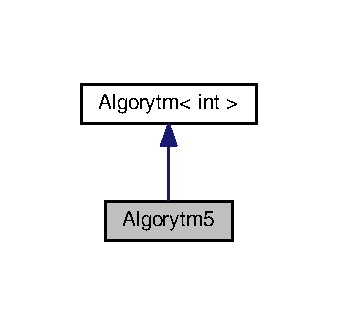
\includegraphics[width=162pt]{a00116}
\end{center}
\end{figure}


Collaboration diagram for Algorytm5\+:
\nopagebreak
\begin{figure}[H]
\begin{center}
\leavevmode
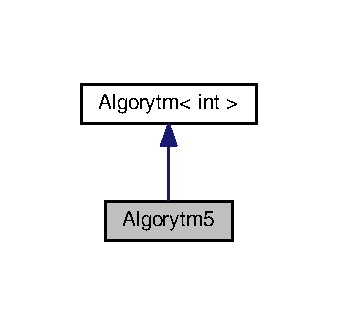
\includegraphics[width=162pt]{a00117}
\end{center}
\end{figure}
\subsection*{Public Member Functions}
\begin{DoxyCompactItemize}
\item 
void \hyperlink{a00006_a9e0b784c6d35486bd95ad063dd40a9b1}{alokujdane} (\hyperlink{a00017}{Zasobnik}$<$ int $>$ $\ast$, int $\ast$, int)
\begin{DoxyCompactList}\small\item\em Metoda alokujaca na zasobniku dane. \end{DoxyCompactList}\item 
void \hyperlink{a00006_ae6b796569be801a1f5816b7bbd700fa3}{wykonajalgorytm} (\hyperlink{a00017}{Zasobnik}$<$ int $>$ $\ast$, int $\ast$, int)
\begin{DoxyCompactList}\small\item\em Metoda wykonujaca konkretny algorytm. \end{DoxyCompactList}\end{DoxyCompactItemize}


\subsection{Detailed Description}
Klasa \hyperlink{a00006}{Algorytm5}. 

\subsection{Member Function Documentation}
\hypertarget{a00006_a9e0b784c6d35486bd95ad063dd40a9b1}{}\index{Algorytm5@{Algorytm5}!alokujdane@{alokujdane}}
\index{alokujdane@{alokujdane}!Algorytm5@{Algorytm5}}
\subsubsection[{alokujdane}]{\setlength{\rightskip}{0pt plus 5cm}void Algorytm5\+::alokujdane (
\begin{DoxyParamCaption}
\item[{{\bf Zasobnik}$<$ int $>$ $\ast$}]{Tab, }
\item[{int $\ast$}]{dane, }
\item[{int}]{liczba\+\_\+danych}
\end{DoxyParamCaption}
)\hspace{0.3cm}{\ttfamily [virtual]}}\label{a00006_a9e0b784c6d35486bd95ad063dd40a9b1}


Metoda alokujaca na zasobniku dane. 


\begin{DoxyParams}{Parameters}
{\em Tab} & -\/ typu Zasobnik$<$\+T$>$$\ast$, implementacja zasobnika \\
\hline
{\em dane} & -\/ typu T$\ast$, dane wygenerowane dla implementacji \\
\hline
{\em liczba\+\_\+danych} & -\/ typu int, liczba danych dla zasobnika \\
\hline
\end{DoxyParams}


Implements \hyperlink{a00001_a1e83fd87a20fd0a13ebbf1c81e457b61}{Algorytm$<$ int $>$}.

\hypertarget{a00006_ae6b796569be801a1f5816b7bbd700fa3}{}\index{Algorytm5@{Algorytm5}!wykonajalgorytm@{wykonajalgorytm}}
\index{wykonajalgorytm@{wykonajalgorytm}!Algorytm5@{Algorytm5}}
\subsubsection[{wykonajalgorytm}]{\setlength{\rightskip}{0pt plus 5cm}void Algorytm5\+::wykonajalgorytm (
\begin{DoxyParamCaption}
\item[{{\bf Zasobnik}$<$ int $>$ $\ast$}]{Tab, }
\item[{int $\ast$}]{dane, }
\item[{int}]{liczba\+\_\+danych}
\end{DoxyParamCaption}
)\hspace{0.3cm}{\ttfamily [virtual]}}\label{a00006_ae6b796569be801a1f5816b7bbd700fa3}


Metoda wykonujaca konkretny algorytm. 


\begin{DoxyParams}{Parameters}
{\em Tab} & -\/ typu Zasobnik$<$\+T$>$$\ast$, implementacja zasobnika \\
\hline
{\em dane} & -\/ typu T$\ast$, dane wygenerowane dla implementacji \\
\hline
{\em liczba\+\_\+danych} & -\/ typu int, liczba danych dla zasobnika \\
\hline
\end{DoxyParams}


Implements \hyperlink{a00001_ae97a52b1a728be1a819c9e9815f424e7}{Algorytm$<$ int $>$}.



The documentation for this class was generated from the following files\+:\begin{DoxyCompactItemize}
\item 
\hyperlink{a00027}{Algorytm5.\+hh}\item 
\hyperlink{a00026}{Algorytm5.\+cpp}\end{DoxyCompactItemize}

\hypertarget{a00007}{}\section{Algorytm6 Class Reference}
\label{a00007}\index{Algorytm6@{Algorytm6}}


Klasa \hyperlink{a00007}{Algorytm6}.  




{\ttfamily \#include $<$Algorytm6.\+hh$>$}



Inheritance diagram for Algorytm6\+:
\nopagebreak
\begin{figure}[H]
\begin{center}
\leavevmode
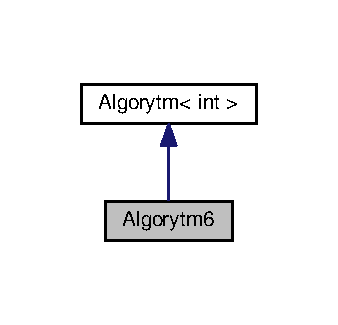
\includegraphics[width=162pt]{a00133}
\end{center}
\end{figure}


Collaboration diagram for Algorytm6\+:
\nopagebreak
\begin{figure}[H]
\begin{center}
\leavevmode
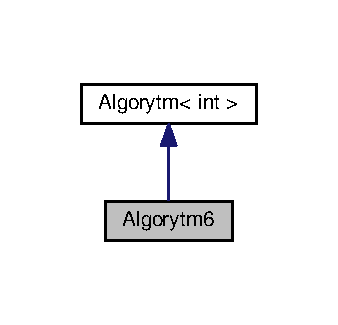
\includegraphics[width=162pt]{a00134}
\end{center}
\end{figure}
\subsection*{Public Member Functions}
\begin{DoxyCompactItemize}
\item 
\hyperlink{a00007_a7b3c905b3b07a0fb8d75b16b64d3246a}{$\sim$\+Algorytm6} ()
\item 
void \hyperlink{a00007_aa655b50c332496def9903e3bd01874d5}{alokujdane} (\hyperlink{a00019}{Zasobnik}$<$ int $>$ $\ast$, int $\ast$, int)
\begin{DoxyCompactList}\small\item\em Metoda alokujaca na zasobniku dane. \end{DoxyCompactList}\item 
void \hyperlink{a00007_afb0db254f1ecc88e80f3e7f19739539c}{wykonajalgorytm} (\hyperlink{a00019}{Zasobnik}$<$ int $>$ $\ast$, int $\ast$, int)
\begin{DoxyCompactList}\small\item\em Metoda wykonujaca konkretny algorytm. \end{DoxyCompactList}\end{DoxyCompactItemize}


\subsection{Detailed Description}
Klasa \hyperlink{a00007}{Algorytm6}. 

\subsection{Constructor \& Destructor Documentation}
\hypertarget{a00007_a7b3c905b3b07a0fb8d75b16b64d3246a}{}\index{Algorytm6@{Algorytm6}!````~Algorytm6@{$\sim$\+Algorytm6}}
\index{````~Algorytm6@{$\sim$\+Algorytm6}!Algorytm6@{Algorytm6}}
\subsubsection[{$\sim$\+Algorytm6}]{\setlength{\rightskip}{0pt plus 5cm}Algorytm6\+::$\sim$\+Algorytm6 (
\begin{DoxyParamCaption}
{}
\end{DoxyParamCaption}
)\hspace{0.3cm}{\ttfamily [inline]}}\label{a00007_a7b3c905b3b07a0fb8d75b16b64d3246a}


\subsection{Member Function Documentation}
\hypertarget{a00007_aa655b50c332496def9903e3bd01874d5}{}\index{Algorytm6@{Algorytm6}!alokujdane@{alokujdane}}
\index{alokujdane@{alokujdane}!Algorytm6@{Algorytm6}}
\subsubsection[{alokujdane}]{\setlength{\rightskip}{0pt plus 5cm}void Algorytm6\+::alokujdane (
\begin{DoxyParamCaption}
\item[{{\bf Zasobnik}$<$ int $>$ $\ast$}]{Tab, }
\item[{int $\ast$}]{dane, }
\item[{int}]{liczba\+\_\+danych}
\end{DoxyParamCaption}
)\hspace{0.3cm}{\ttfamily [virtual]}}\label{a00007_aa655b50c332496def9903e3bd01874d5}


Metoda alokujaca na zasobniku dane. 


\begin{DoxyParams}{Parameters}
{\em Tab} & -\/ typu Zasobnik$<$\+T$>$$\ast$, implementacja zasobnika \\
\hline
{\em dane} & -\/ typu T$\ast$, dane wygenerowane dla implementacji \\
\hline
{\em liczba\+\_\+danych} & -\/ typu int, liczba danych dla zasobnika \\
\hline
\end{DoxyParams}


Implements \hyperlink{a00001_a1e83fd87a20fd0a13ebbf1c81e457b61}{Algorytm$<$ int $>$}.



Here is the call graph for this function\+:
\nopagebreak
\begin{figure}[H]
\begin{center}
\leavevmode
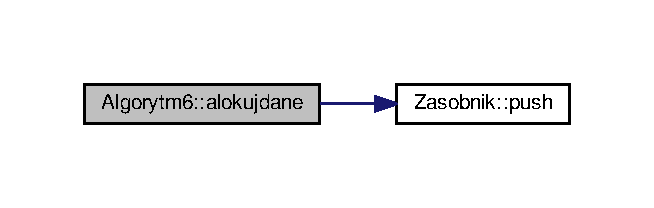
\includegraphics[width=314pt]{a00007_aa655b50c332496def9903e3bd01874d5_cgraph}
\end{center}
\end{figure}


\hypertarget{a00007_afb0db254f1ecc88e80f3e7f19739539c}{}\index{Algorytm6@{Algorytm6}!wykonajalgorytm@{wykonajalgorytm}}
\index{wykonajalgorytm@{wykonajalgorytm}!Algorytm6@{Algorytm6}}
\subsubsection[{wykonajalgorytm}]{\setlength{\rightskip}{0pt plus 5cm}void Algorytm6\+::wykonajalgorytm (
\begin{DoxyParamCaption}
\item[{{\bf Zasobnik}$<$ int $>$ $\ast$}]{Tab, }
\item[{int $\ast$}]{dane, }
\item[{int}]{liczba\+\_\+danych}
\end{DoxyParamCaption}
)\hspace{0.3cm}{\ttfamily [virtual]}}\label{a00007_afb0db254f1ecc88e80f3e7f19739539c}


Metoda wykonujaca konkretny algorytm. 


\begin{DoxyParams}{Parameters}
{\em Tab} & -\/ typu Zasobnik$<$\+T$>$$\ast$, implementacja zasobnika \\
\hline
{\em dane} & -\/ typu T$\ast$, dane wygenerowane dla implementacji \\
\hline
{\em liczba\+\_\+danych} & -\/ typu int, liczba danych dla zasobnika \\
\hline
\end{DoxyParams}


Implements \hyperlink{a00001_ae97a52b1a728be1a819c9e9815f424e7}{Algorytm$<$ int $>$}.



Here is the call graph for this function\+:
\nopagebreak
\begin{figure}[H]
\begin{center}
\leavevmode
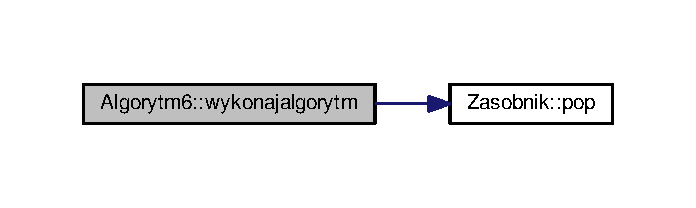
\includegraphics[width=334pt]{a00007_afb0db254f1ecc88e80f3e7f19739539c_cgraph}
\end{center}
\end{figure}




The documentation for this class was generated from the following files\+:\begin{DoxyCompactItemize}
\item 
\hyperlink{a00031}{Algorytm6.\+hh}\item 
\hyperlink{a00030}{Algorytm6.\+cpp}\end{DoxyCompactItemize}

\hypertarget{a00008}{\section{Benchmark.\-cpp File Reference}
\label{a00008}\index{Benchmark.\-cpp@{Benchmark.\-cpp}}
}


Metody klasy \hyperlink{a00002}{Benchmarker}.  


{\ttfamily \#include \char`\"{}Benchmark.\-hh\char`\"{}}\\*
{\ttfamily \#include \char`\"{}Lista.\-hh\char`\"{}}\\*
{\ttfamily \#include \char`\"{}Stos.\-hh\char`\"{}}\\*
{\ttfamily \#include \char`\"{}Kolejka.\-hh\char`\"{}}\\*
{\ttfamily \#include \char`\"{}Array\-Lista.\-hh\char`\"{}}\\*
{\ttfamily \#include $<$cstdlib$>$}\\*
{\ttfamily \#include $<$iostream$>$}\\*
{\ttfamily \#include $<$ctime$>$}\\*
Include dependency graph for Benchmark.\-cpp\-:\nopagebreak
\begin{figure}[H]
\begin{center}
\leavevmode
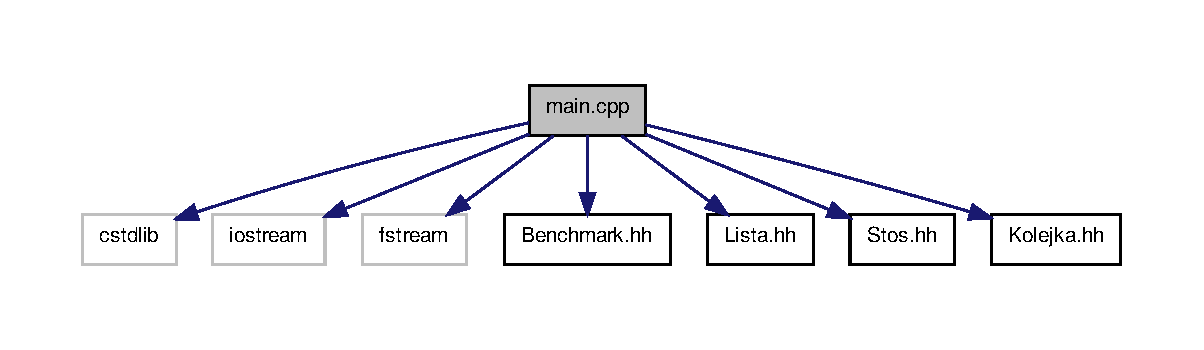
\includegraphics[width=350pt]{a00022}
\end{center}
\end{figure}
\subsection*{Macros}
\begin{DoxyCompactItemize}
\item 
\#define \hyperlink{a00008_af899221e0ac3b868dd9a8298bd9b1f12}{B\-E\-N\-C\-H\-M\-A\-R\-K\-\_\-\-C\-P\-P}
\end{DoxyCompactItemize}


\subsection{Detailed Description}
Metody klasy \hyperlink{a00002}{Benchmarker}. Plik zawiera metody klasy \hyperlink{a00002}{Benchmarker}. 

\subsection{Macro Definition Documentation}
\hypertarget{a00008_af899221e0ac3b868dd9a8298bd9b1f12}{\index{Benchmark.\-cpp@{Benchmark.\-cpp}!B\-E\-N\-C\-H\-M\-A\-R\-K\-\_\-\-C\-P\-P@{B\-E\-N\-C\-H\-M\-A\-R\-K\-\_\-\-C\-P\-P}}
\index{B\-E\-N\-C\-H\-M\-A\-R\-K\-\_\-\-C\-P\-P@{B\-E\-N\-C\-H\-M\-A\-R\-K\-\_\-\-C\-P\-P}!Benchmark.cpp@{Benchmark.\-cpp}}
\subsubsection[{B\-E\-N\-C\-H\-M\-A\-R\-K\-\_\-\-C\-P\-P}]{\setlength{\rightskip}{0pt plus 5cm}\#define B\-E\-N\-C\-H\-M\-A\-R\-K\-\_\-\-C\-P\-P}}\label{a00008_af899221e0ac3b868dd9a8298bd9b1f12}

\hypertarget{a00009}{}\section{Benchmarker$<$ T $>$ Class Template Reference}
\label{a00009}\index{Benchmarker$<$ T $>$@{Benchmarker$<$ T $>$}}


Szablon klasy \hyperlink{a00009}{Benchmarker}.  




{\ttfamily \#include $<$Benchmark.\+hh$>$}



Inheritance diagram for Benchmarker$<$ T $>$\+:
\nopagebreak
\begin{figure}[H]
\begin{center}
\leavevmode
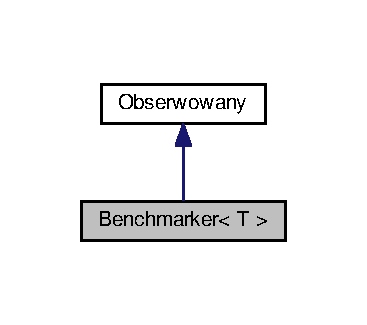
\includegraphics[width=176pt]{a00139}
\end{center}
\end{figure}


Collaboration diagram for Benchmarker$<$ T $>$\+:
\nopagebreak
\begin{figure}[H]
\begin{center}
\leavevmode
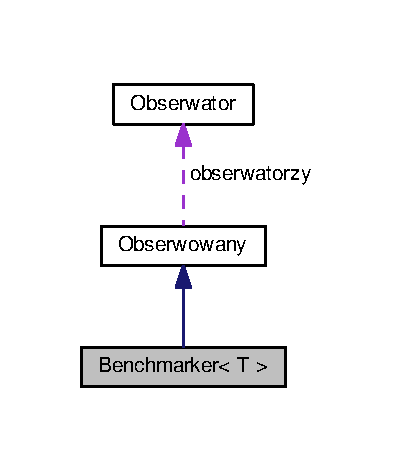
\includegraphics[width=190pt]{a00140}
\end{center}
\end{figure}
\subsection*{Public Member Functions}
\begin{DoxyCompactItemize}
\item 
void \hyperlink{a00009_aeecfb553991fc29bbf58420d0c019c1e}{testuj} (\hyperlink{a00019}{Zasobnik}$<$ T $>$ $\ast$, \hyperlink{a00001}{Algorytm}$<$ T $>$ $\ast$, T $\ast$, int, int)
\begin{DoxyCompactList}\small\item\em Szablon metody przeprowadzajaca sprawdzenie czasu dzialania funkcji. Typy\+: \hyperlink{a00014}{Lista} , \hyperlink{a00018}{Stos} , \hyperlink{a00013}{Kolejka}, \hyperlink{a00012}{Hasz\+Tab}. \end{DoxyCompactList}\item 
void \hyperlink{a00009_a6d9c92477ce398fc8ec38b24f49fa9a1}{powiadom} (int, long int)
\begin{DoxyCompactList}\small\item\em Metoda powiadamiajaca obserwatora o czasie wykonania. \end{DoxyCompactList}\end{DoxyCompactItemize}
\subsection*{Additional Inherited Members}


\subsection{Detailed Description}
\subsubsection*{template$<$typename T$>$class Benchmarker$<$ T $>$}

Szablon klasy \hyperlink{a00009}{Benchmarker}. 

\subsection{Member Function Documentation}
\hypertarget{a00009_a6d9c92477ce398fc8ec38b24f49fa9a1}{}\index{Benchmarker@{Benchmarker}!powiadom@{powiadom}}
\index{powiadom@{powiadom}!Benchmarker@{Benchmarker}}
\subsubsection[{powiadom}]{\setlength{\rightskip}{0pt plus 5cm}template$<$typename T $>$ void {\bf Benchmarker}$<$ T $>$\+::powiadom (
\begin{DoxyParamCaption}
\item[{int}]{iteracja, }
\item[{long int}]{czas\+\_\+sredni}
\end{DoxyParamCaption}
)}\label{a00009_a6d9c92477ce398fc8ec38b24f49fa9a1}


Metoda powiadamiajaca obserwatora o czasie wykonania. 


\begin{DoxyParams}{Parameters}
{\em iteracja} & -\/ typu int, liczba danych -\/ identyfikator iteracji \\
\hline
{\em czas\+\_\+sredni} & -\/ typu long int, czas wykonania operacji \\
\hline
\end{DoxyParams}
\hypertarget{a00009_aeecfb553991fc29bbf58420d0c019c1e}{}\index{Benchmarker@{Benchmarker}!testuj@{testuj}}
\index{testuj@{testuj}!Benchmarker@{Benchmarker}}
\subsubsection[{testuj}]{\setlength{\rightskip}{0pt plus 5cm}template$<$typename T $>$ template void {\bf Benchmarker}$<$ T $>$\+::testuj (
\begin{DoxyParamCaption}
\item[{{\bf Zasobnik}$<$ T $>$ $\ast$}]{, }
\item[{{\bf Algorytm}$<$ T $>$ $\ast$}]{, }
\item[{T $\ast$}]{, }
\item[{int}]{, }
\item[{int}]{}
\end{DoxyParamCaption}
)}\label{a00009_aeecfb553991fc29bbf58420d0c019c1e}


Szablon metody przeprowadzajaca sprawdzenie czasu dzialania funkcji. Typy\+: \hyperlink{a00014}{Lista} , \hyperlink{a00018}{Stos} , \hyperlink{a00013}{Kolejka}, \hyperlink{a00012}{Hasz\+Tab}. 


\begin{DoxyTemplParams}{Template Parameters}
{\em Tab} & -\/ typu T$\ast$, wskaznik na zaimplementowany stos/liste/kolejke/tablice haszującą. \\
\hline
{\em dane} & -\/ typu int$\ast$, wskaznik na tablice z danymi generowanymi. \\
\hline
{\em liczba\+\_\+przejsc} & -\/ typu int, liczba przejsc przez dane. \\
\hline
{\em liczba\+\_\+danych} & -\/ typu int, liczba danych w tablicy. \\
\hline
\end{DoxyTemplParams}
\begin{DoxyReturn}{Returns}
czas\+\_\+calkowity\+\_\+usredniony -\/ typu long int, czas sredni dzialania funkcji. 
\end{DoxyReturn}


Here is the call graph for this function\+:
\nopagebreak
\begin{figure}[H]
\begin{center}
\leavevmode
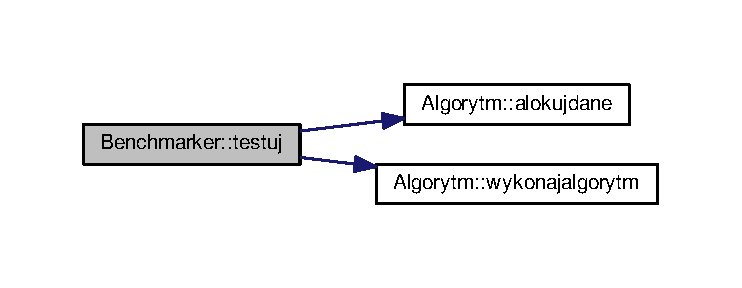
\includegraphics[width=350pt]{a00009_aeecfb553991fc29bbf58420d0c019c1e_cgraph}
\end{center}
\end{figure}




The documentation for this class was generated from the following files\+:\begin{DoxyCompactItemize}
\item 
\hyperlink{a00036}{Benchmark.\+hh}\item 
\hyperlink{a00035}{Benchmark.\+cpp}\end{DoxyCompactItemize}

\hypertarget{a00010}{}\section{Benchmark.\+hh File Reference}
\label{a00010}\index{Benchmark.\+hh@{Benchmark.\+hh}}


Definicja klasy \hyperlink{a00002}{Benchmarker}.  


{\ttfamily \#include $<$string$>$}\\*
Include dependency graph for Benchmark.\+hh\+:\nopagebreak
\begin{figure}[H]
\begin{center}
\leavevmode
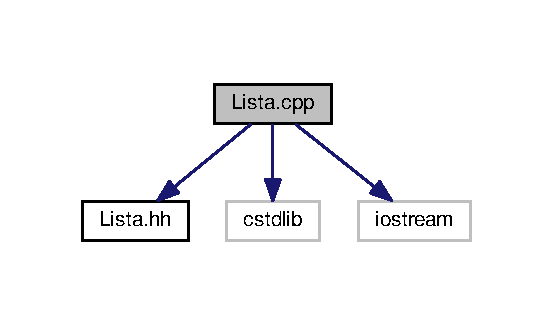
\includegraphics[width=160pt]{a00026}
\end{center}
\end{figure}
This graph shows which files directly or indirectly include this file\+:\nopagebreak
\begin{figure}[H]
\begin{center}
\leavevmode
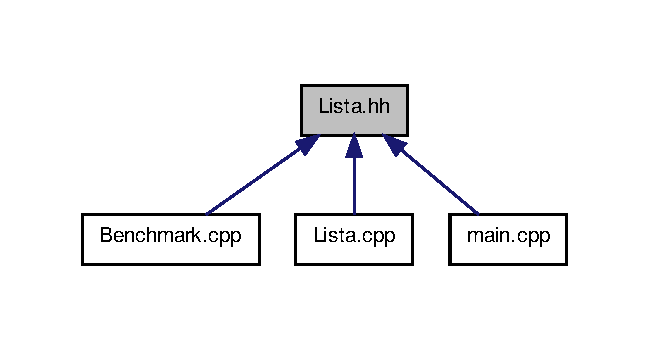
\includegraphics[width=239pt]{a00027}
\end{center}
\end{figure}
\subsection*{Classes}
\begin{DoxyCompactItemize}
\item 
class \hyperlink{a00002}{Benchmarker}
\begin{DoxyCompactList}\small\item\em Klasa \hyperlink{a00002}{Benchmarker}. \end{DoxyCompactList}\end{DoxyCompactItemize}


\subsection{Detailed Description}
Definicja klasy \hyperlink{a00002}{Benchmarker}. 

Plik zawiera definicje klasy \hyperlink{a00002}{Benchmarker}. 
\hypertarget{a00011}{}\section{Hasz\+Tab.\+cpp File Reference}
\label{a00011}\index{Hasz\+Tab.\+cpp@{Hasz\+Tab.\+cpp}}


Metody klasy \hyperlink{a00003}{Hasz\+Tab}.  


{\ttfamily \#include \char`\"{}Hasz\+Tab.\+hh\char`\"{}}\\*
{\ttfamily \#include $<$cstdlib$>$}\\*
{\ttfamily \#include $<$iostream$>$}\\*
Include dependency graph for Hasz\+Tab.\+cpp\+:\nopagebreak
\begin{figure}[H]
\begin{center}
\leavevmode
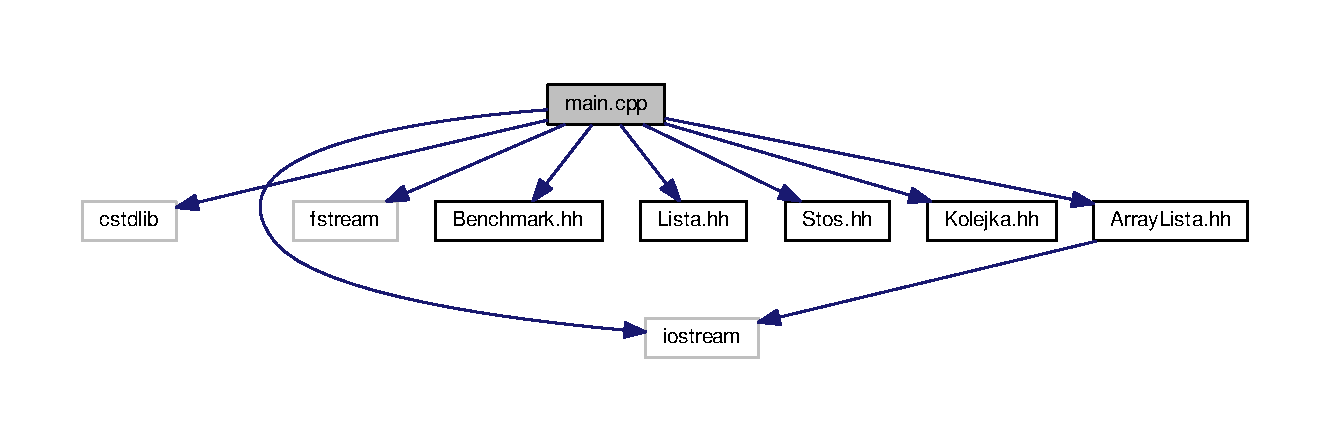
\includegraphics[width=268pt]{a00028}
\end{center}
\end{figure}


\subsection{Detailed Description}
Metody klasy \hyperlink{a00003}{Hasz\+Tab}. 

Plik zawiera metody klasy \hyperlink{a00003}{Hasz\+Tab}. 
\hypertarget{a00012}{\section{Stos.\-cpp File Reference}
\label{a00012}\index{Stos.\-cpp@{Stos.\-cpp}}
}


Metody klasy \hyperlink{a00004}{Stos}.  


{\ttfamily \#include \char`\"{}Stos.\-hh\char`\"{}}\\*
{\ttfamily \#include $<$cstdlib$>$}\\*
{\ttfamily \#include $<$iostream$>$}\\*
Include dependency graph for Stos.\-cpp\-:\nopagebreak
\begin{figure}[H]
\begin{center}
\leavevmode
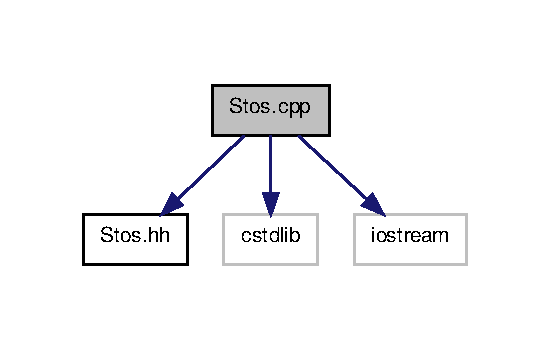
\includegraphics[width=264pt]{a00023}
\end{center}
\end{figure}


\subsection{Detailed Description}
Metody klasy \hyperlink{a00004}{Stos}. Plik zawiera metody klasy \hyperlink{a00004}{Stos}. 
\hypertarget{a00013}{\section{Lista.\-hh File Reference}
\label{a00013}\index{Lista.\-hh@{Lista.\-hh}}
}


Definicja klasy \hyperlink{a00004}{Lista}.  


This graph shows which files directly or indirectly include this file\-:\nopagebreak
\begin{figure}[H]
\begin{center}
\leavevmode
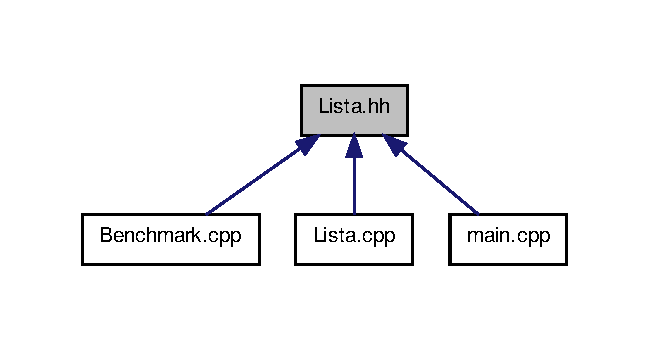
\includegraphics[width=312pt]{a00027}
\end{center}
\end{figure}
\subsection*{Classes}
\begin{DoxyCompactItemize}
\item 
class \hyperlink{a00004}{Lista}
\begin{DoxyCompactList}\small\item\em Klasa \hyperlink{a00004}{Lista}. \end{DoxyCompactList}\end{DoxyCompactItemize}


\subsection{Detailed Description}
Definicja klasy \hyperlink{a00004}{Lista}. Plik zawiera definicje klasy modulujacej pojecie listy jednokierunkowej. 
%--- End generated contents ---

% Index
\newpage
\phantomsection
\addcontentsline{toc}{section}{Index}
\printindex

\end{document}
